\documentclass[12pt]{article}
\usepackage{graphicx}

\title{Geometr\'{\i}as lineales (Prueba evaluaci\'on continua)}
\date{2019-11-30}
\author{Javier Garc\'{\i}a Parra}

\begin{document}
    \maketitle
    \newpage



    A partir de la transformaci\'on de los puntos  P en P\textquotesingle y Q en Q\textquotesingle, \\
    las matrices de las isometr\'{\i}as deben ser de la forma (M):\\

    $$\pmatrix{1&0&0\cr a&{{1}\over{2}}&{{1}\over{2}}\cr b&{{\sqrt{3}
    }\over{2}}&{{1}\over{2}}\cr }$$

    Con un polinomio caracter\'{\i}stico del tipo:

    $$-{{\left(t-1\right)\,\left(4\,t^2-4\,t-\sqrt{3}+1\right)}\over{4}}$$

    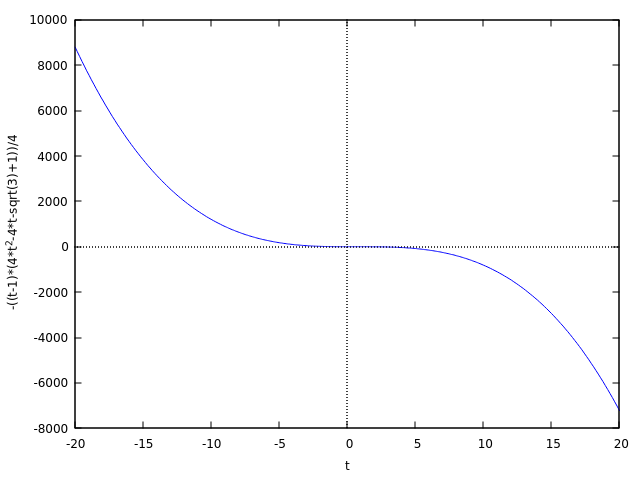
\includegraphics{polinomio_caracteristico.png}

    Observ\'andolo, parece que la isometr\'{\i}a ser\'a una reflexi\'on con deslizamiento.

    La forma de Jordan ser\'a de la forma:

    $$\pmatrix{-{{3^{{{1}\over{4}}}-1}\over{2}}&0&0\cr 0&{{3^{{{1}\over{4
    }}}+1}\over{2}}&0\cr 0&0&1\cr }$$

    En las notas adjuntas, se desarrolla el c\'alculo del vector de desplazamiento y del eje de rotaci\'on de la isometr\'{\i}a.

    Tambi\'en se adjunta el script main.mac, desarrollado para contrastar los resultados con maxima.
\end{document}
